

\documentclass[10pt,a4paper]{article}
\usepackage[utf8]{inputenc}
\usepackage[english]{babel}
\usepackage{amsmath}
\usepackage{amsfonts}
\usepackage{amssymb}
\usepackage{graphicx}
\usepackage{caption}
\usepackage{float}
\usepackage{array}
\usepackage{booktabs}	% for horizontal lines
\usepackage{varwidth}% http://ctan.org/pkg/varwidth
\usepackage{csvsimple} % automatic table generation from csv files
\usepackage{comment}
\usepackage[style=draft, backend=biber]{biblatex}

\addbibresource{../bibliography.bib}

\title{Experiments}
\author{Weber Jakob}

\begin{document}
	\maketitle
	
\section{Simulations}

Following the descriptions given in the previous chapters, we are now going to test the algorithm of structured additive regression using a priori knowledge on the following problems:	

\begin{itemize}
	\item Static Function Approximation using a priori Knowledge
	\item Equidistant vs. Non-equidistant Knot Placement
	\item Different Levels and Colors of Noise $\lambda^2$
	\item Well-distributed Data vs. Skewed Data
\end{itemize}

These are evaluated on two functions with a priori known behavior. The first function is given by
\begin{equation} \label{eq:test_func_1}
	f(x) = \begin{cases}
			 0 \quad &\text{if} \ x \le 0.8 \\ 
			 20\sin (x-1.2) \quad &\text{else}  
		  \end{cases}, \quad \text{for} \ x \in [0,2.5]. \quad 
\end{equation}
	
It is therefor a constant function till $x=0.8$ and afterwards increasing. An example of the true function as well as noisy samples from this function is given in Fig. \ref{eq:test_func_1}.

\begin{figure}[H]
	\centering
	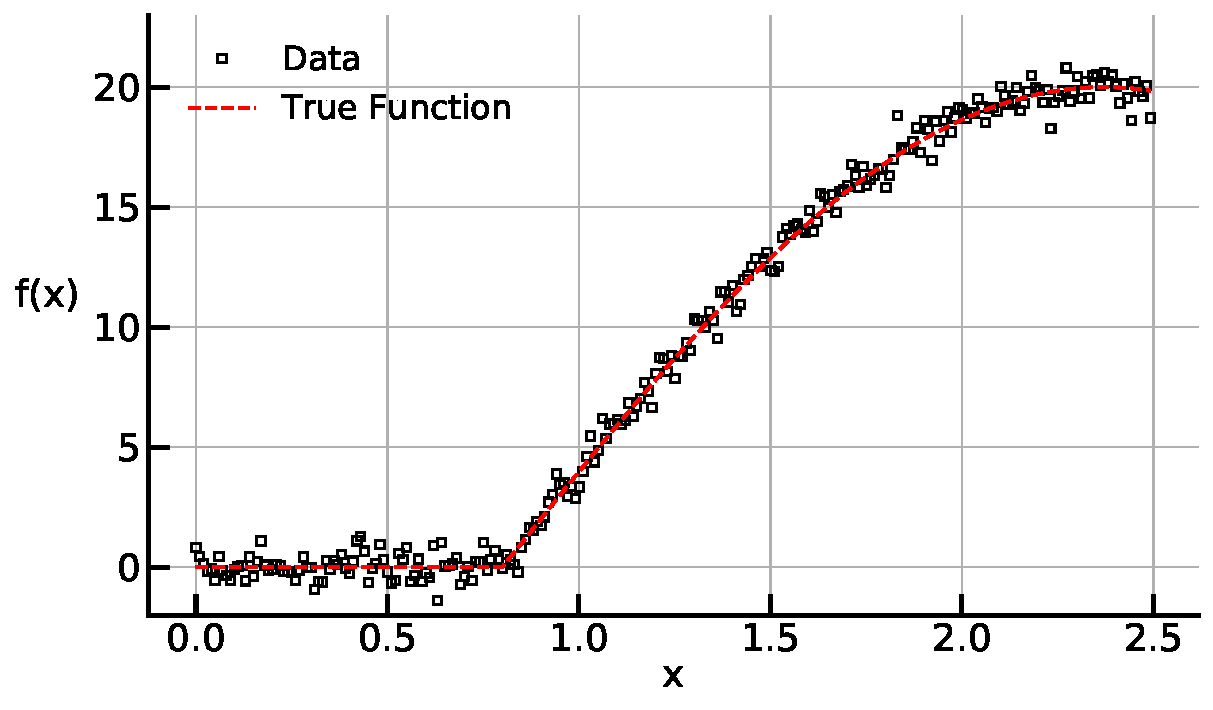
\includegraphics[width=\columnwidth]{../thesisplots/exp_inc1.pdf}
	\caption{Test Function 1}
	\label{fig:test_func_1}
\end{figure}

The second function that will be investigated is given by
\begin{equation} \label{eq:test_func_2}
	f(x) = 2\exp \big(-\frac{(x-0.5)^2}{0.05} \big) + 2.5x, \quad \text{for} \ x \in [0,1]
\end{equation}

We therefor use the a priori knowledge that the function is unimodal. An example of the true function as well as noisy samples is given in the following figure.

\begin{figure}[H]
	\centering
	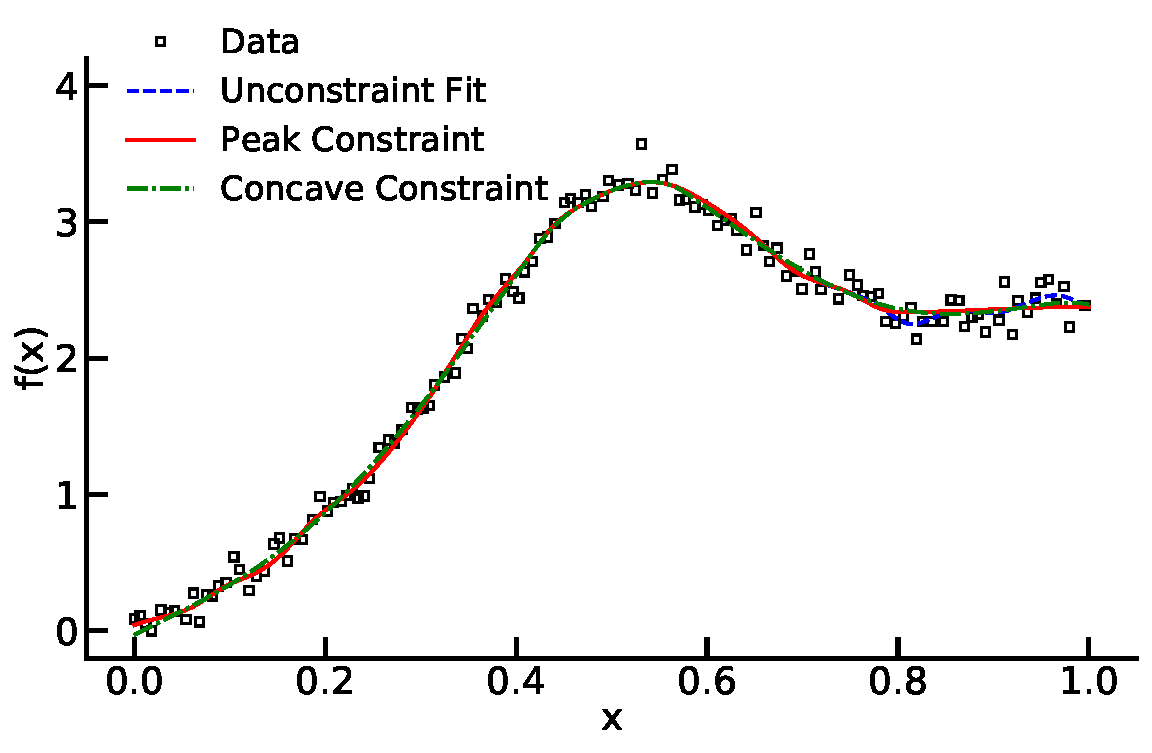
\includegraphics[width=\columnwidth]{../thesisplots/exp_peak1.pdf}
	\caption{Test Function 2}
	\label{fig:test_func_2}
\end{figure}

\subsection{Static Function Approximation using a priori Knowledge}

For the test using function \ref{eq:test_func_1}, the data set contains 1000 points. We use $k=35$ as number of used splines. The smoothing parameter $\lambda_s$ is optimized using cross-validation. The parameter regulating the influence of the constraint is set to the 1000-fold of the smoothing parameter $\lambda_s$. The resulting constrained fit, and for comparison, the unconstrained fit using the optimal smoothing parameter $\lambda_s = 4.15$ are shown in the following figure.

\begin{figure}[H]
	\centering
	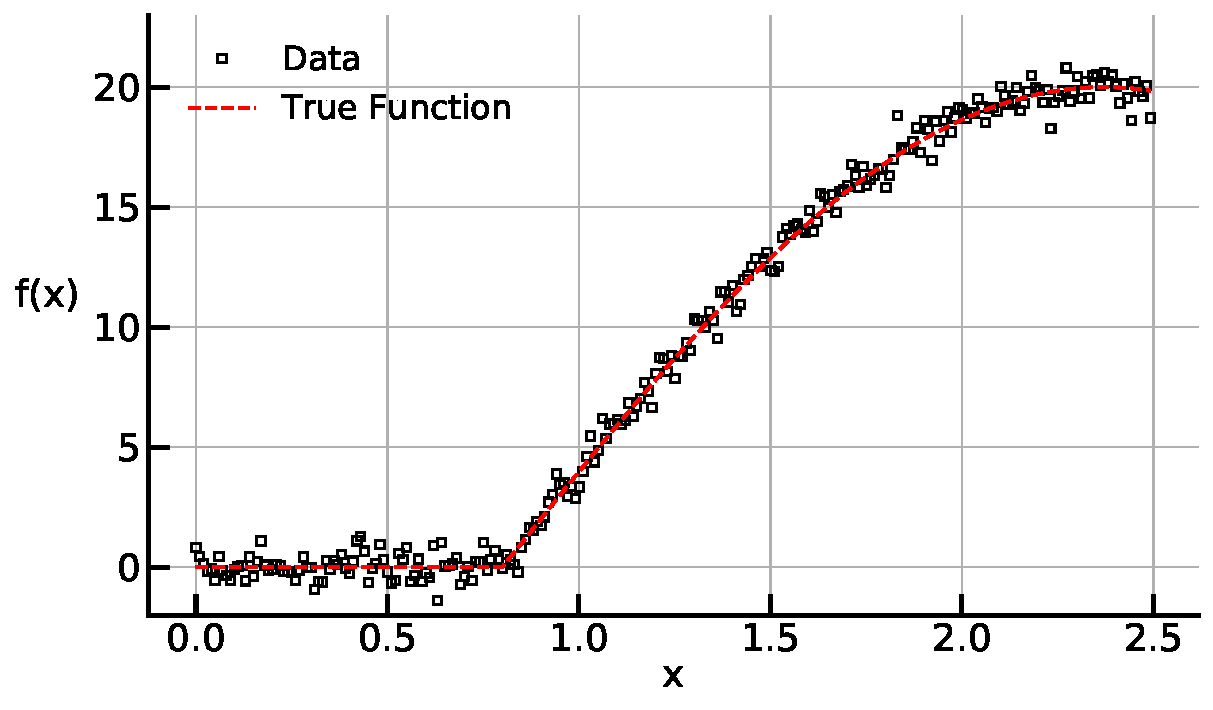
\includegraphics[width=\columnwidth]{../thesisplots/exp_inc1.pdf}
	\caption{Constrained and Unconstrained Fit for Test Function 1}
	\label{fig:fit_test_func_1}
\end{figure}

The red line follows the a priori knowledge of increasing behavior better than the blue, unconstrained line. Especially in the constant area, e.g. $x \in  [0, 1]$ and $x > 2.5$, the constraint improves the static function approximation. In the area of increasing behavior, the two fits are almost identical. The mean squared error on the training data, on the test data and on the true function are given in the Table Results.

For the test using function \ref{eq:test_func_2} the data set contains 500 points. There are two possibilities to include the a priori knowledge of a peak. First we can use the peak constraint matrix given in Chapter Penalty Matrices. On the other hand, we can simply use the concavity constraint, since concave functions are likely to have a peak when the data shows a peak. We examine both possibilities in the following figure. For each fit, we used $k=35$ as number of used splines and the smoothing parameter $\lambda_s = 1.2115$ was again optimized using cross-validation. The constraint parameter $\lambda_c$ was set equal to 1211.5.

\begin{figure}[H]
	\centering
	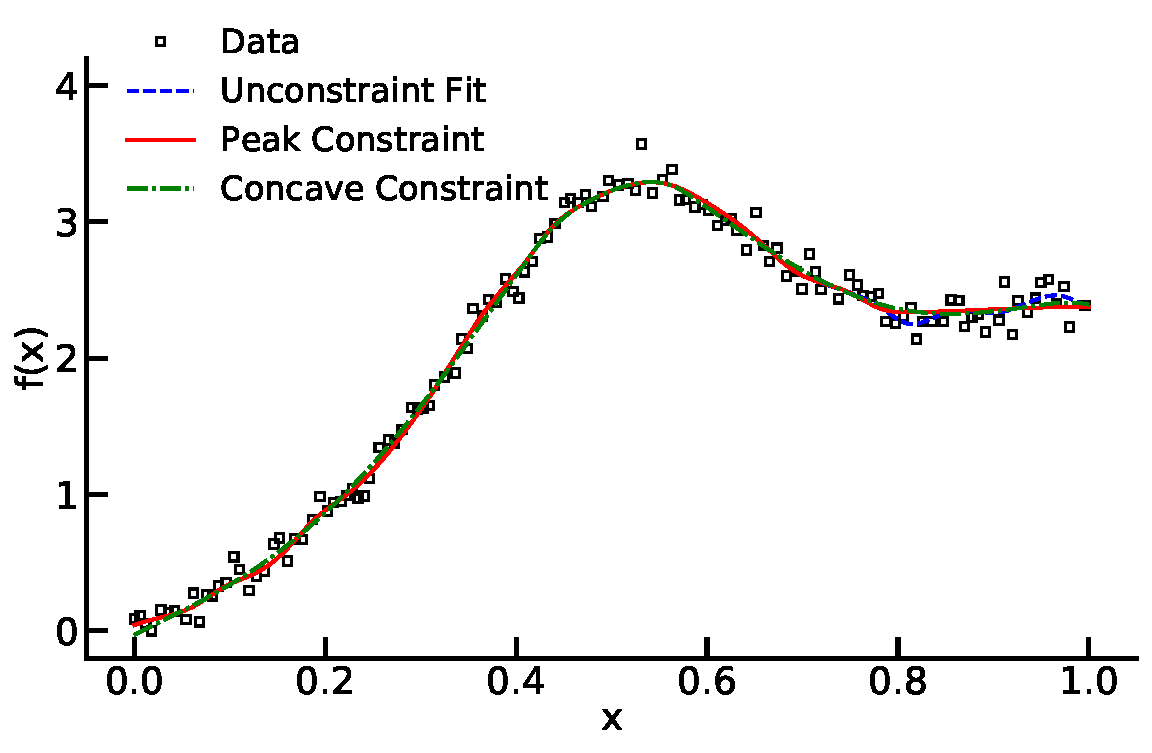
\includegraphics[width=\columnwidth]{../thesisplots/exp_peak1.pdf}
	\caption{Test Function 2}
	\label{fig:fit_test_func_2}
\end{figure}
 
The estimate for the concave constraint shows a the desired peak behavior, and is more smooth than the peak constraint estimate. The peak constraint identifies the peak correctly and produces a sufficiently smooth fit. The mean squared errors are given in the results table. 
It is important to notice that the concavity constraint must be used carefully, since not all functions with a peak are also concave or vice versa.

\subsection{Constraint vs. Noise}

In this section, we investigate the effect of different noise levels as well as noise types on the fitting process. In the first part, various levels of Gaussian noise are applied to function \ref{eq:test_func_2}. In the second part, we will use different colors of noise acting on function \ref{eq:test_func_1}. For both examples we use $k=35$ splines and optimize the smoothing parameter $\lambda_s$ using cross-validation. 

\subsubsection{Noise Level}

Gaussian noise is characterized by the following two parameters:
\begin{itemize}
	\item Location: The mean value $\mu$ of the Gaussian distribution.
	\item Scale: The variance value $\sigma^2$ of the Gaussian distribution.
\end{itemize}

We set the location equal to zero and vary the scale value. The effect of the noise on the fitting procedure is shown in the following figure. The chosen noise levels are $\sigma^2 = \{0.01, 0.05, 0.1\}$.

For these values of $\sigma^2$, the correspond optimized smoothing parameters are $\lambda_{0.01} = 9.0$, $\lambda_{0.05} = \lambda_{0.1} = 68.1$.

\begin{figure}[H]
	\centering
	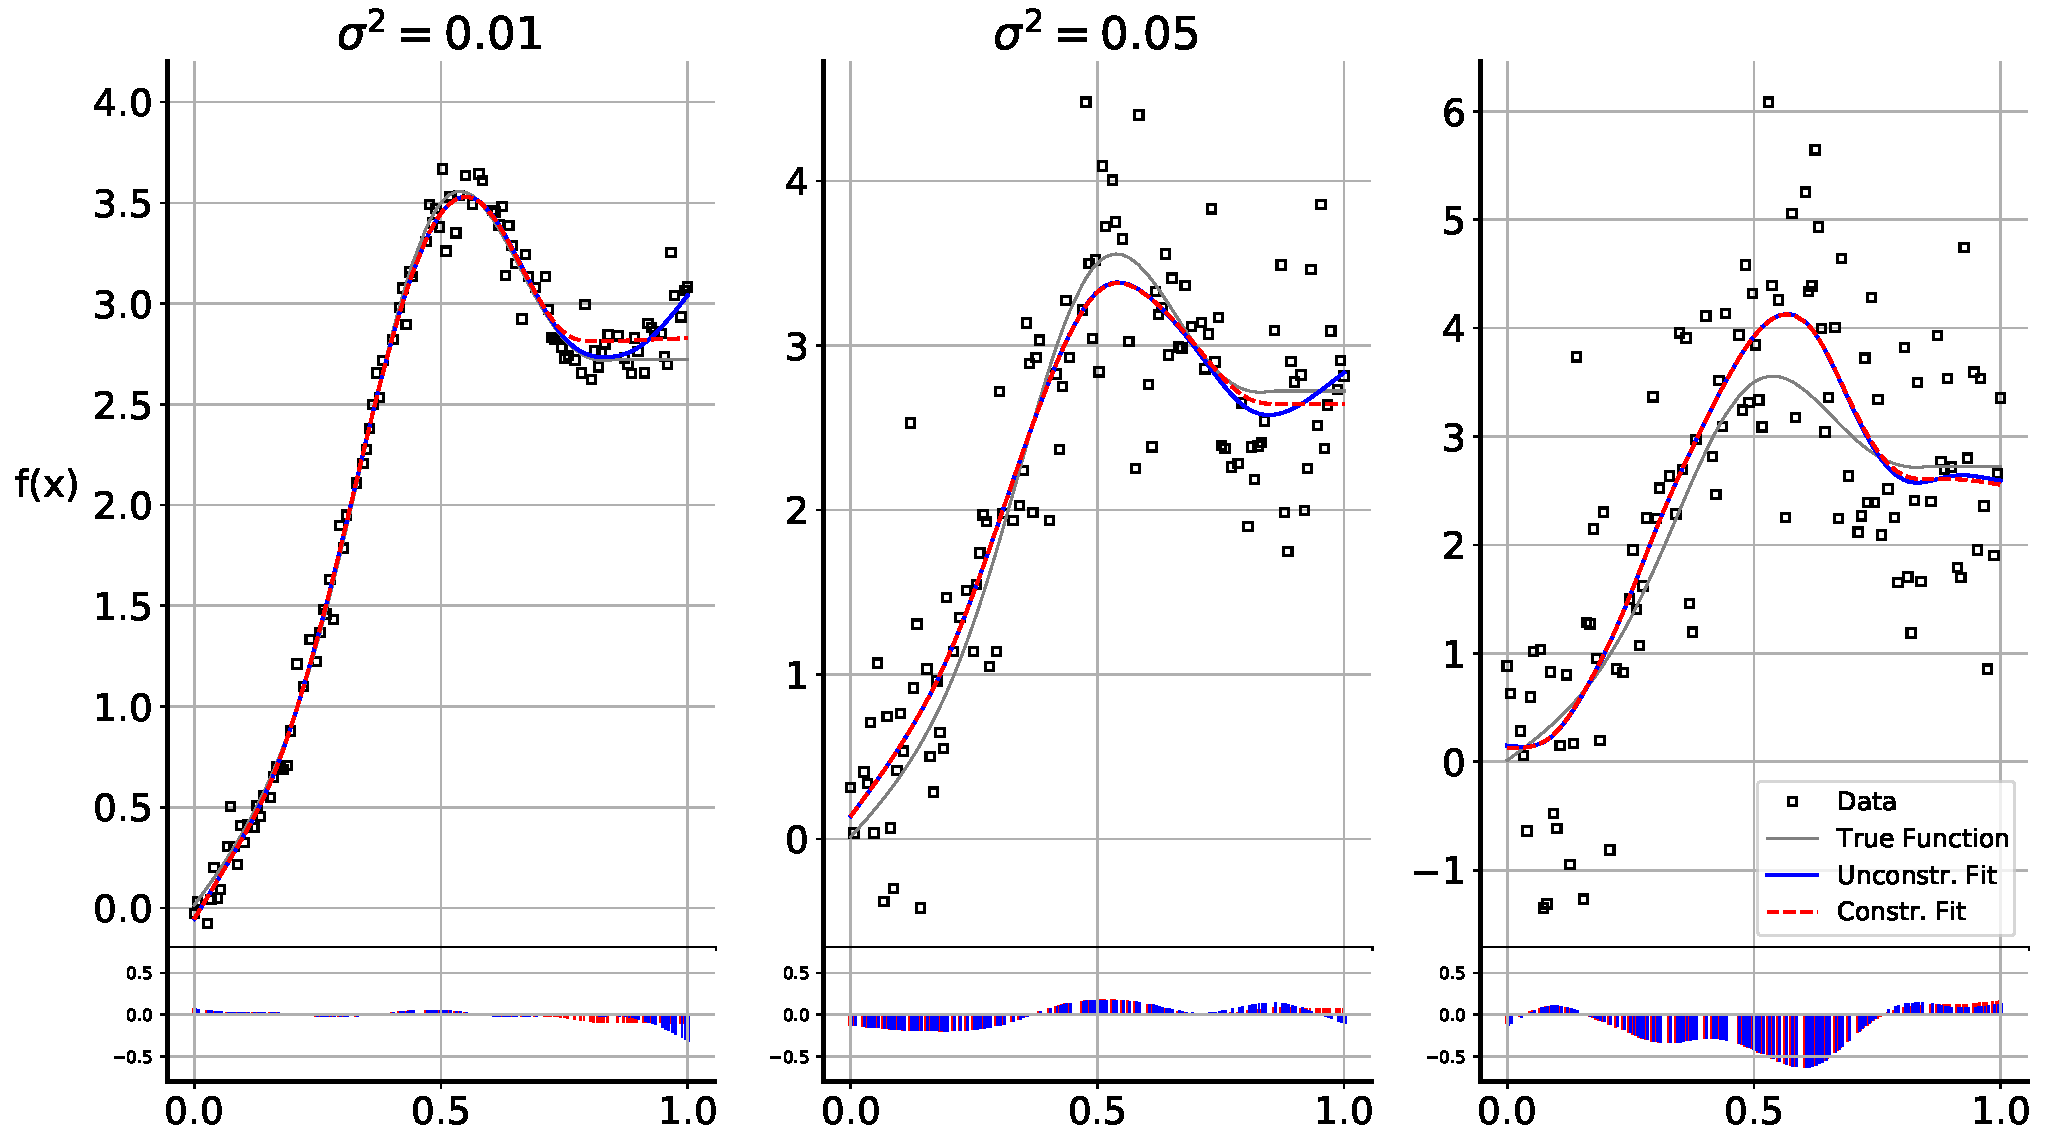
\includegraphics[width=\columnwidth]{../thesisplots/exp_noise_levels.pdf}
	\caption{Constrained and Unconstraint Fit for various Noise Levels}
	\label{fig:fit_noise_levels}
\end{figure}

The left plot shows the fit for $\sigma^2 = 0.01$. The noise level is quite moderate, which leads to a smooth and satisfying fit. The peak constraint is well satisfied. The constraint parameter $\lambda_c$ was set to $\lambda_c = 1000\lambda_s$. 

The noise level in the middle plot is already high. The unconstrained fit is therefore wiggly and shows 2 peaks. The constrained fit holds the peak constraint and generalizes better to the test set, as seen in *table resulst MSES.* The constraint parameter was again set to $\lambda_c = 1000\lambda_s.$ 

For the right plot and $\sigma^2=0.1$, both constrained and unconstrained fit are wiggly but for larger $x$, the constraint fit follows the constraint better. The constraint parameter was set to $\lambda_c = 1000\lambda_s$.

\subsubsection{Noise Colors}

We investigate the effect of different noise color on the function fitting process. The tested colors are the following power-law noise types:

\begin{itemize}
	\item  White Noise
	\item Pink Noise
	\item Brownian Noise
\end{itemize}

The unconstrained as well as the increasing constrained fit for all noise colors are shown in the following figure.

\begin{figure}[H]
	\centering
	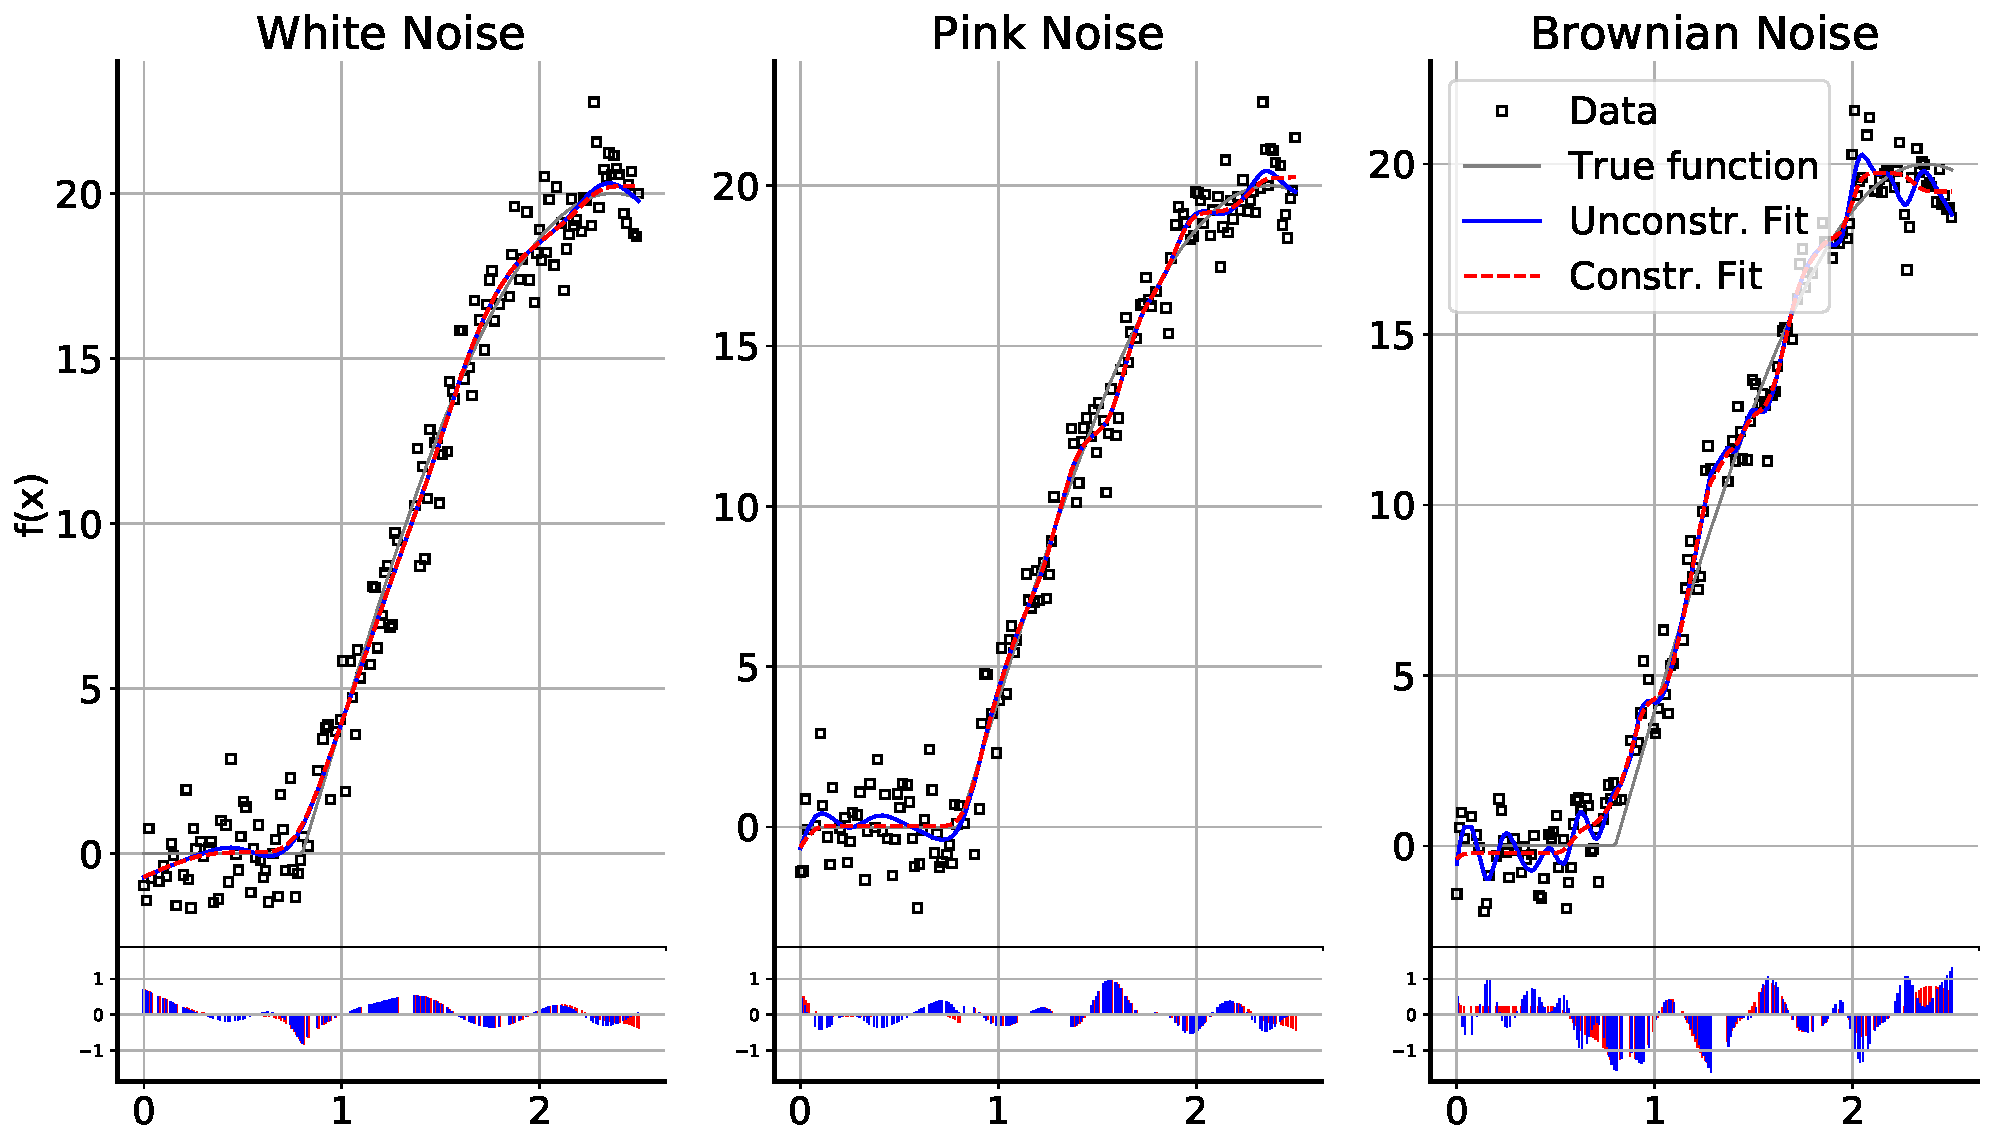
\includegraphics[width=\columnwidth]{../thesisplots/exp_noise_colors.pdf}
	\caption{Constrained and Unconstrained Fit for various Noise Colors}
	\label{fig:fit_noise_colors}
\end{figure}

For the white noise data in the left plot, the increasing constraint produces a very good fit according to the constraint. The optimized smoothing parameter for the unconstrained fit was given by $\lambda_s = 9.08$ and the constraint parameter was set to $\lambda_c = 9080$. The fit recovers the true function quite well. 

For the pink noise data in the middle plot, the constraint helps regularizing the fit, but the increasing constraint is not satisfied especially for low $x$. The increasing part of the function, i.e. $f(x)$ for $x \ge 1.2$,  was fit well. The smoothing parameter was optimized using cross-validation and set to $\lambda_s = 0.3$. The constraint parameter was set to $\lambda_c = 6000$. 

For the brownian noise data in the right plot, the increasing part of the function was fit well, but for larger $x \ge 2$, the fit diverges the true function because of the strong noise component. The increasing constraint is hold quite well. The optimized smoothing parameter used was $\lambda_s = 0.0056$ and the constraint parameter was set to $\lambda_c = 6000$.

\subsection{Well-distributed vs. Skewed Data and Knot Placement}


\begin{itemize}
	\item Phasendiagram: $\sigma^2 vs. \lambda_c$
	\item Ebner Data
\end{itemize}

\end{document}